%%% -*-LaTeX-*-

\chapter{Implemention Details}

This chapter examines the implementation and encoding decisions.

\section{Language Implementation: Decisions and Alternatives}

SweetPea is an embedded domain specific language, meaning that instead of providing its own syntax and the compiler infrastructure to match, it is instead implemented as a library in an embedding language. Here we look at the choice of embedding language, as well as some choices about boolean encodings.

\subsection{Embedding Language}

The current implementation of SweetPea is embedded in Python; the syntax presented in the example code snippets in chapter 4 are valid python program snippets. The subsystem for handling Tsietin transforms is currently implemented in Haskell; an earlier implementation of the user-facing SweetPea syntax was also implemented in Haskell. We chose Haskell as an implementation language because its strong static types and functional purity lent it to verifying the correctness of the system. However, many scientists are familiar with Python, and not with Haskell syntax, so we decided to port the user-facing interface to Python to make it easier for them to use and interface with their existing workflows.

\section{Communicating with the SAT-Sampler}

\figref{fig_architecture} illustrates SweetPea's current architecture. It is more complicated than a single executable. This is partially because part of the constraints are generated by a Python program and part by the Haskell subsystem, and partially because the SAT sampler that SweetPea calls out to, Unigen, only runs on POSIX compliant systems (Linux, but not MacOS). Because of both of these facts, SweetPea is a python program which runs, and calls out to, a docker container. This docker container consists of the Haskell subsystem which can efficiently encode counting constraints, and unigen, which takes the constraints that the program compiled to and produce a satisfying assignment, should one exist.

\begin{figure}[t]
    \centerline{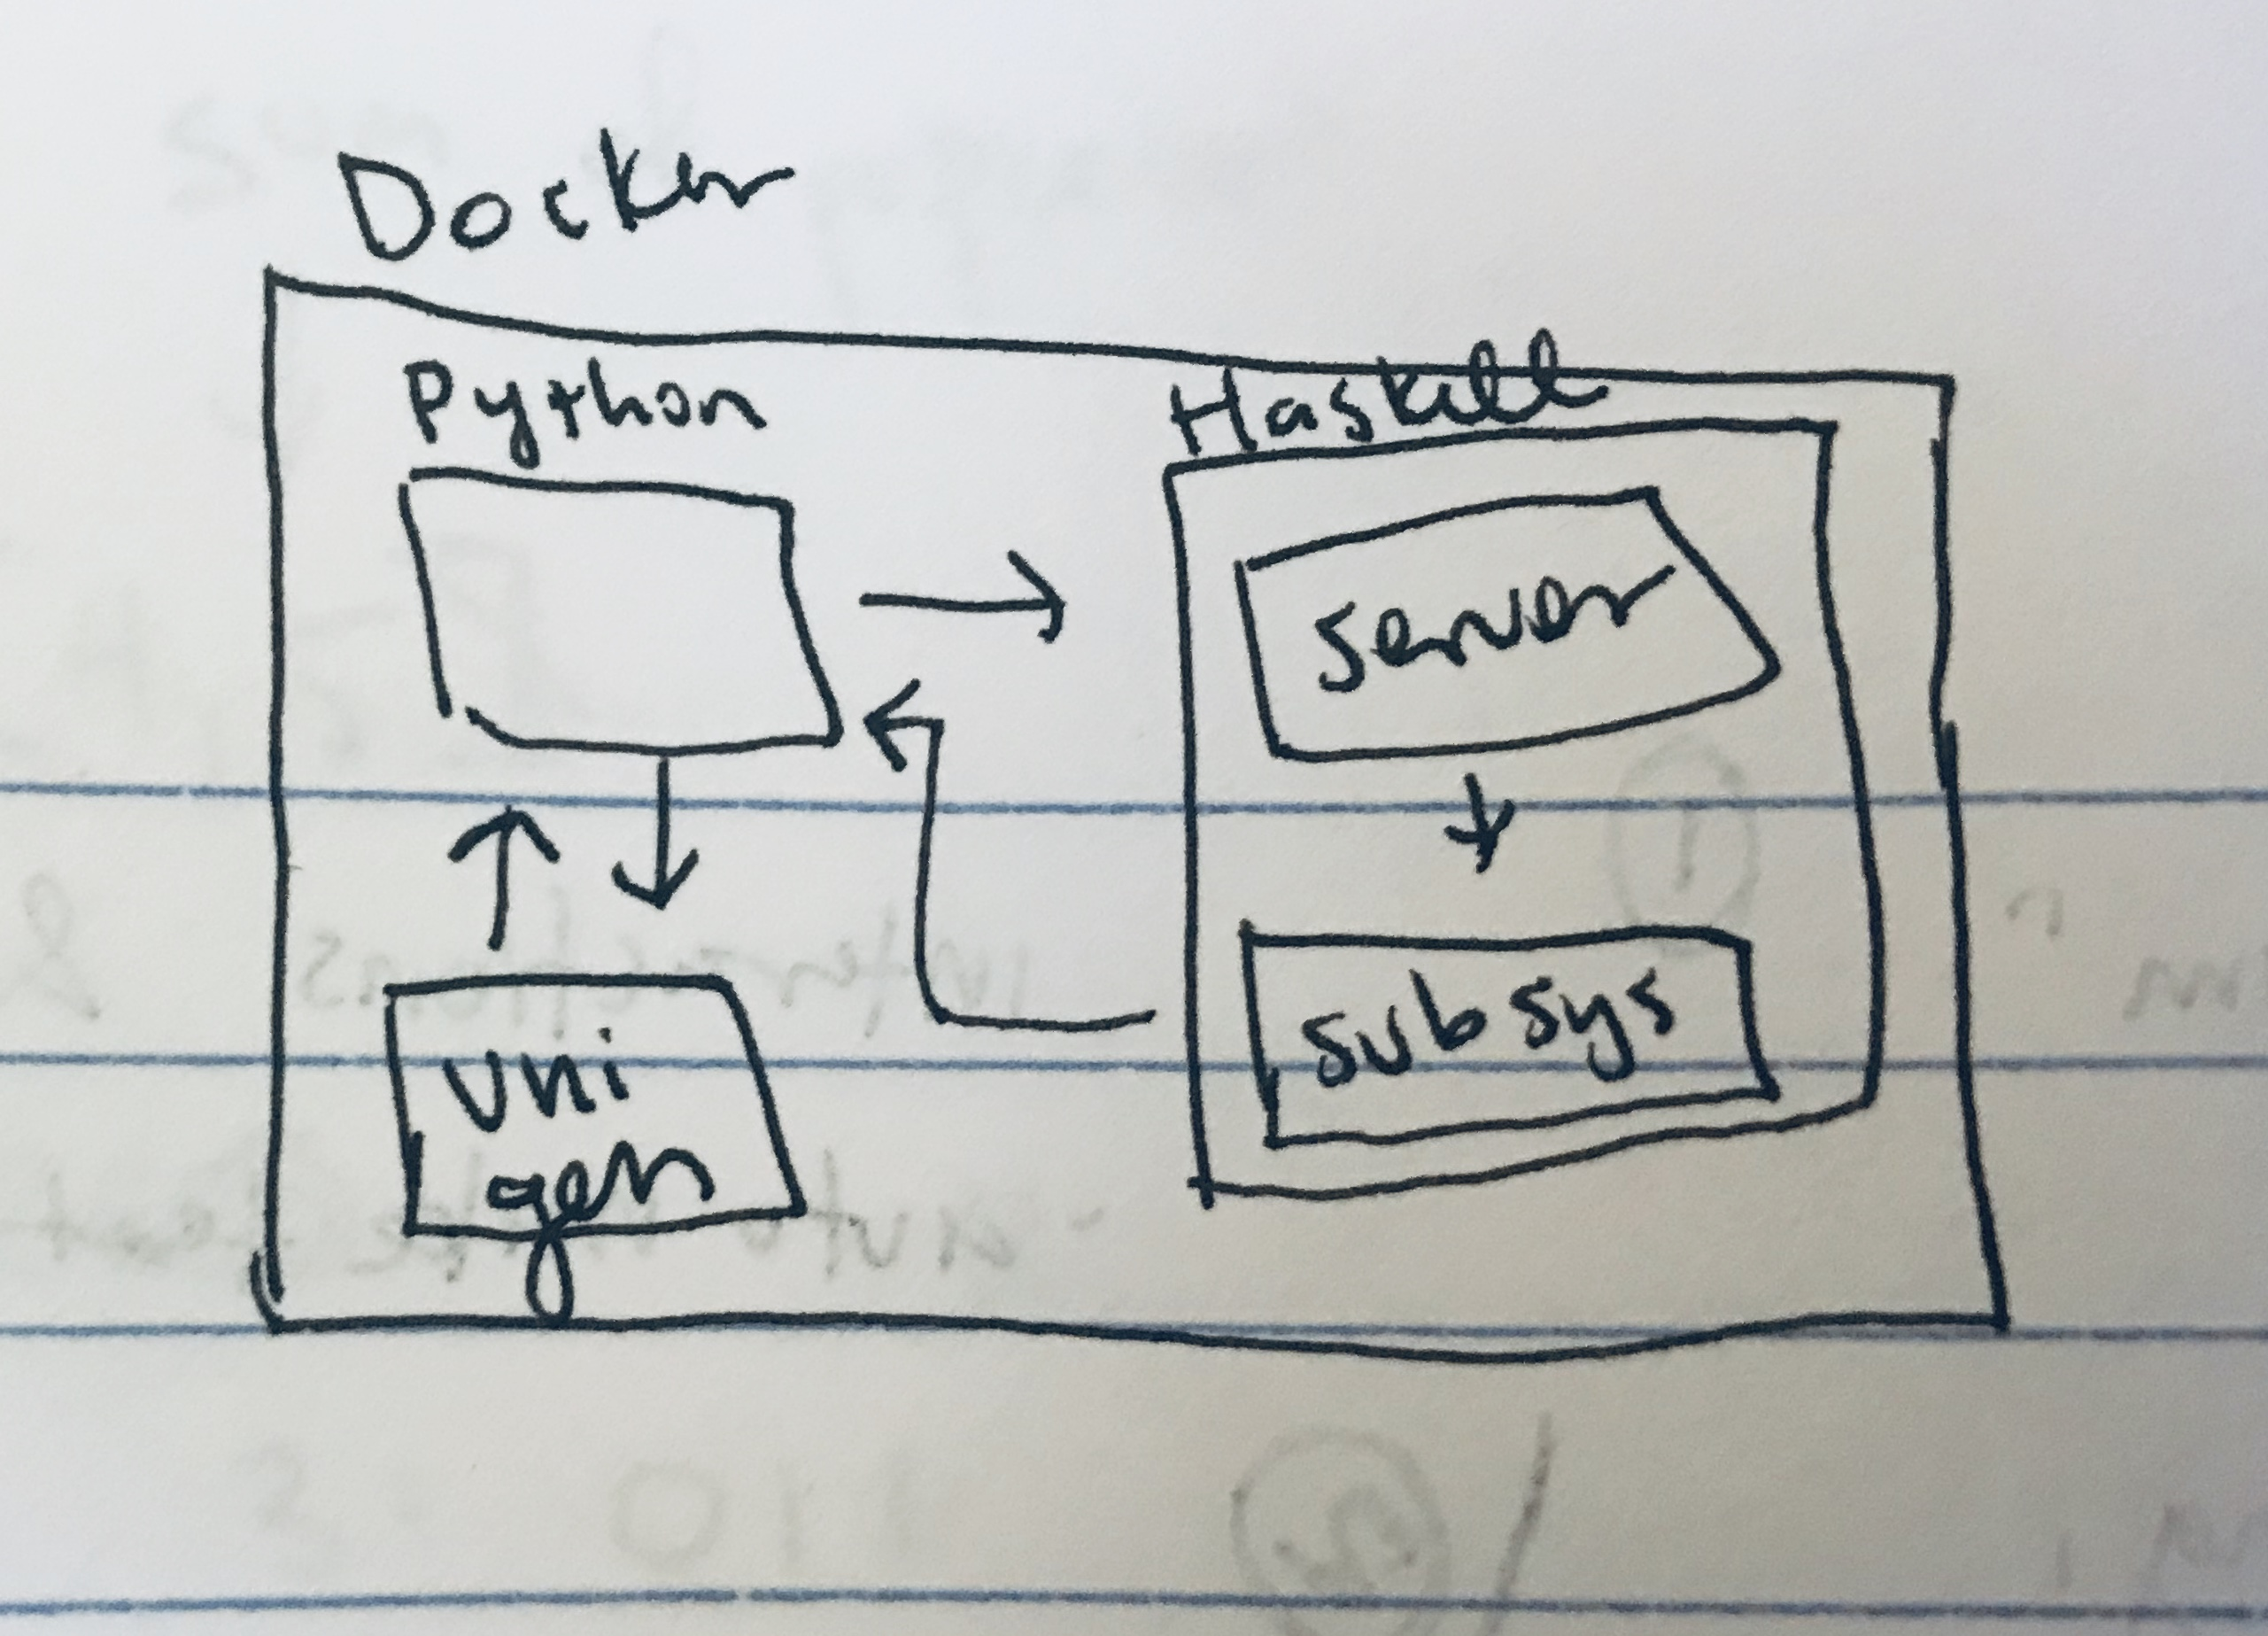
\includegraphics[origin=c,width=7cm]{fig_architecture}}
    \caption{Architecture of SweetPea deployment.}%
    \label{fig:fig_architecture}%
\end{figure}

Unigen provides two features in addition to the standard DIMACS format: the ability to denote which variables are "important" for a final assignment (in our case, those that directly encode the state of the experimental sequence), and the ability to provide xors rather than or clauses. The current version of SweetPea uses the first feature (the important variables are called the \emph{supports}), and does not use the second, though it is an optimization for future work.

After SweetPea, the python program which called out to the docker container, gets a response from unigen, it translates it back to a human-readable format. This means translating the assignments to the experimental sequence they represent (see \figref{example_assignment} for an example). The resulting sequence can either be printed as a list of strings, or can be exported to a list of python dictionaries to be directly integrated into other psychology computational tools such as psyNeuLink.

\subsection{Internal Representations}

As mentioned in the previous chapter, we encode levels by allocating one boolean variable per level to indicate the whether that level is in a selected or unselected state. This isn't the only possible


- pros / cons of using one-hot vs binary : trade-off between more variables and more clauses

- todo: more examples

\section{Encoding Counting Constraints: Tsietin Transform}
\cite{tseitin1983complexity}

A fully crossed design specifies that each possible combination of levels occurs once in the design. A realistic experiment may have 7 factors, with 2 levels each, for a total of $2^7$ = 128 trials. Each of the levels will appear in half the trials, which means we need to encode constraints of the form "exactly 64 of these 128 variables must be true". The naive encoding ("these 64, or those 64, or those 64, etc") will have 64 choose 128 clauses, which is $10^{37}$ clauses-- far more than any SAT solver can possibly handle. Therefore, we need to encode these kinds of counting constraints in an encoding which is linear in the number of clauses and variables.

To achieve this linear encoding, we emulate the logic in a \emph{popcount} circuit. A popcount circuit is a piece of hardware built out of logic gates which, given a bit string, reports how many bits of the bit string are set. A popcount circuit is implemented as a series of multi-bit wide adders. To explain how we emulate the logic in these circuits we will start with adders and build up to the popcount circuit.

\subsection{Adders}

TODO diagrams: 1) half-adder, 2) visualization of 1+1, 3) full-adder 4) ripple carry adder
TODO solver v sampler
TODO maybe actual DIMACS half adder that you can run

First let's consider a half-adder. A half-adder is a circuit which takes two single bit inputs a and b and sets two single bit outputs s ("sum") and c ("carry") according to what the sum of the values of a and b are. The value of the input bits is 1 if that variable is true, and 0 if that variable is false. The output bits are boolean functions of the input bits: s = a xor b ; c = a and b.

What does it mean for a boolean variable to "equal" some relationship between other boolean variables? Really what we mean here is that their values vary in lock-step; that the variable being bound is true only when the relation is true, and false identically when the relation is false. This is the boolean relation iff. This means that we can represent a half-adder with the boolean formula:
(s iff (a xor b)) and (c iff (a and b)).

How does using a SAT solver allow us to emulate this circuit? Recall that the solver's job is to return an assignment to each of our variables (a, b, c, s) such that the entire formula.

Let's look at some examples. Lets imagine adding 1 + 1; this means that the full formula we hand to the solver is:
(s iff (a xor b)) and (c iff (a and b)) and (a) and (b).
For the entire formula to be true, each of the and clauses must be true. This trivially means that the assignment for a is true, and b is true. Looking at the more interesting clauses, we know s is true iff (a xor b). a xor b is False when both a and b are true, so s must be false for that clause to be true. We also know that c is true iff (a and b), so c must also be true.

This means that for this input, the solver would give us the satisfying assignment:
a is true
b is true
s is false
c is true

We can interpret this to mean that the carry bit is 1, and the sum bit is 0: meaning that 1 + 1 = 2. The rest of the constructions in this section follow this intuition: if we build up logical relationships between boolean variables which emulate circuits which perform the computation we wish perform, and constrain some of the input variables, then SAT solver will find what the values of all the other variables must be.

In practice, we want to use a full-adder rather than a half-adder; the difference is that a full-adder also considers a "carry in" bit. This makes it possible to chain full-adder together into multi-bit wide adders.

There are multiple ways to chain together multiple full-adders. SweetPea uses the simplest option, which is ripple-carry adders. N-bit wide ripple-carry adders chain together n full-adders in the natural way:

Alternative ways to build multi-bit adders include carry-lookahead adders and carry-save adders; these circuits were designed as physical circuits which can compute the result of the addition in fewer cycles. In some sense, we are also concerned with how long it takes to compute the result: we would like to use the encodings which are most helpful for the solver. There isn't any reason to believe that using a more complicated multi-bit adder design would result in a more favorable encoding; therefore we decided to use the multi-adder design which is simplest to implement, maintain and debug.

\subsection{Pop Count Circuit}

TODO popcount diagram


- pop count circuit example



\subsection{Exhaustive Testing}

- example of input / output: see how it's prone to error

- tested for a given size all assignments
